%!TEX root = ../lections.tex
Рассмотрим уравнение простой волны
\begin{equation}
	\pdv{u}{t}+u\pdv{u}{x}+\beta \pdv[3]{u}{x}-\underbrace{\nu\pdv[2]{u}{x}}_{\text{диссипация}}=0.
	\label{eq:shock:1}
\end{equation}

Здесь $\nu>0$ -- диссипация. Посмотрим, к чему приведет её учет. Если $\beta=0$, то уравнение называется уравнением Бюргерса. 

Будем искать решения в виде $\xi=x-Vt$ (их ещё называют стационарными решениями, так как профиль волны не меняется): 
\begin{equation*}
	-V\dv{u}{\xi}+u\dv{u}{\xi}+\beta\dv[3]{u}{\xi}-\nu\dv[2]{u}{\xi}=0.
\end{equation*}
Проинтегрируем:
\begin{equation*}
	\beta\dv[2]{u}{\xi}-\nu \dv{u}{\xi}+\frac{u^2}{2}-Vu=0.
\end{equation*}
Перепишем полученное уравнение в виде системы, дифференцирование по $\xi$ обозначая точкой:
\begin{equation}
	\begin{cases}
		\dot{u}=y \\
		\beta \dot{y} =\nu y-\frac{u^2}{2}+Vu.		
	\end{cases}
	\label{eq:shock:2}
\end{equation}

Система диссипативная. Найдем её состояния равновесия: $O_1(0,0)$, $O_2(2V,0)$. Несложный анализ (линеаризация) даст, что $O_1$ -- седло, а для $O_2$:
\begin{gather*}
	p^2-\frac{\nu}{\beta}p+\frac{V}{\beta}=0, \qquad p_{1,2}=\frac{\nu}{2\beta}\pm \sqrt{\frac{\nu^2}{4\beta^2}-\frac{V}{\beta}}.
\end{gather*}
Если $\frac{\nu^2}{4\beta^2}-\frac{V}{\beta}<0$, то имеем неустойчивый фокус.
\begin{equation*}
	\frac{\nu^2}{4\beta}=V \quad\rightarrow\quad \beta=\frac{\nu^2}{4V}.
\end{equation*}
Над этой кривой $\beta(\nu)$ состояние равновесия $O_2$ будет неустойчивым фокусом, а под -- неустойчивым узлом (см. рисунок ниже).
\begin{figure}[H]
	\centering
	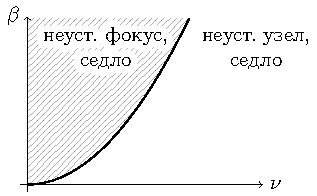
\includegraphics[scale=1.4]{img/shock_waves/beta_nu}
	\caption{Разбиение области параметров}
\end{figure}

Введем в рассмотрение функцию (полную энергию при $\nu=0$)
% Возьмем полную энергию при $\nu=0$:
\begin{equation*}
	V(u,y)=\beta\frac{y^2}{2}+\frac{u^3}{6}-V\frac{u^2}{2},
\end{equation*}
Линии уровня этой функции дают фазовый портрет при $\nu=0$.  Из существования этой функции следует, что система не имеет предельных циклов. 
Найдём производную $\dot{V}$ в силу системы \eqref{eq:shock:2}:
\begin{equation*}
	\dot{V}=\beta y \dot{y}+\frac{u^2}{2}\dot{u}-Vu\dot{u}=\nu y^2-\frac{u^2}{2}y+Vuy-Vuy+\frac{u^2}{2}y=\nu y^2\geqslant 0,
\end{equation*}
т.е. траектории системы пересекают линии уровня в сторону возрастания:
\begin{figure}[H]
	\centering
	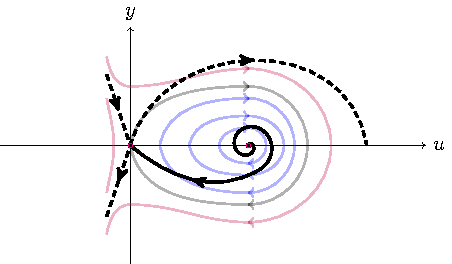
\includegraphics[scale=1.5]{img/shock_waves/phase_portrait}
\end{figure}
Как ведут себя устойчивые сепаратрисы седла? Ограниченное решение существует, оно единственно и соответствует траектории из фокуса в седло (см. рис. выше). 



% \begin{figure}[H]
% 	\centering
% 	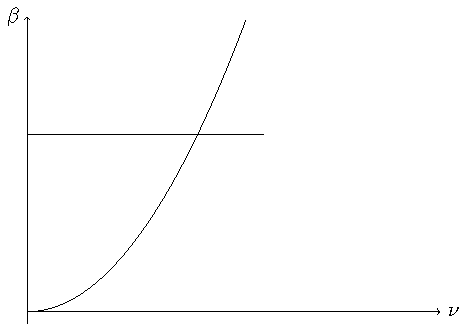
\includegraphics[width=0.4\linewidth]{fig/fig28.pdf}   
% \end{figure}

Зафиксируем $\beta$ и нарисуем профиль этой волны. Будем изучать траекторию, которая успеет сделать много витков, до того как придет в состояние равновесия. По прежнему $\nu\ll1$:
\begin{figure}[H]
	\centering
	% 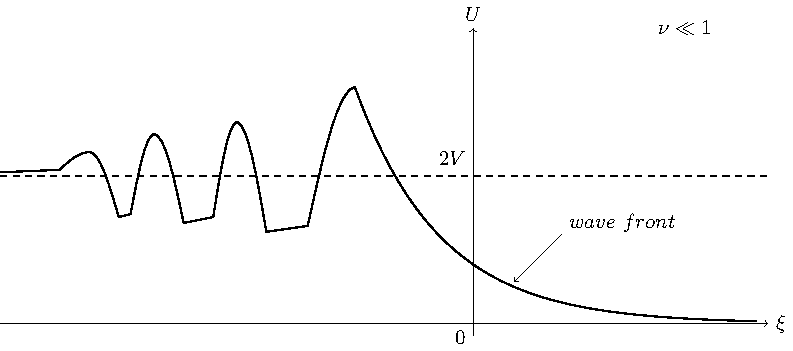
\includegraphics[width=0.6\linewidth]{fig/fig29.pdf} 
	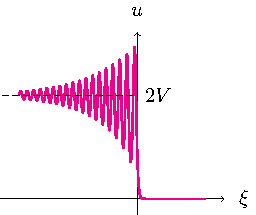
\includegraphics[scale=1.5]{img/shock_waves/shock} 
	\caption{Фронт волны <<переключает>> среду из $2V$ в $0$}
\end{figure}

Чем дальше от седла, тем ближе точки, выше и меньше полки. Это ударная волна.  Среда была в покое, прошел фронт и перебросил среду в новое состояние $2V$.

% Для красной траектории:
% \begin{figure}[H]
% 	\centering
% 	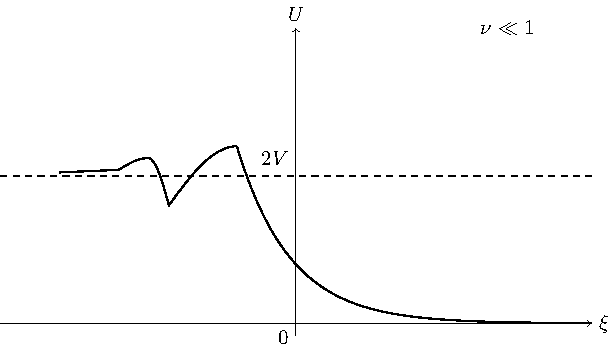
\includegraphics[width=0.6\linewidth]{fig/fig31.pdf}   
% \end{figure}

Если взять такой параметр $\beta$, что состояние равновесия $O_2$ будет узлом, то осцилляций не будет, но передний фронт останется. Волна, соответствующая единственной ограниченной траектории, идущей из неустойчивого состояния равновесия  --  узла в седло:
% \begin{figure}[H]
% 	\centering
% 	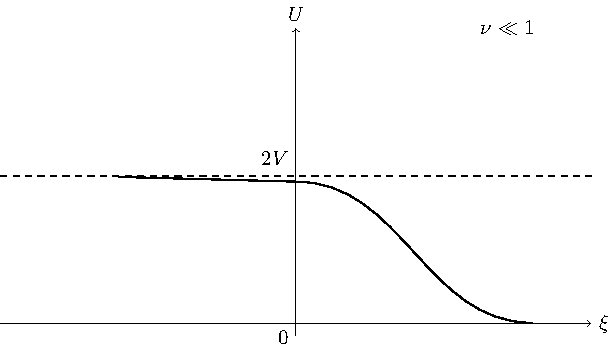
\includegraphics[width=0.6\linewidth]{fig/fig32.pdf}   
% \end{figure}
\begin{figure}[h]
\begin{minipage}[h]{0.49\linewidth}
\center{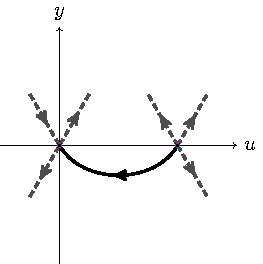
\includegraphics[scale=1.5]{img/shock_waves/phase_portrait_knot}}
\end{minipage}
\hfill
\begin{minipage}[h]{0.49\linewidth}
\center{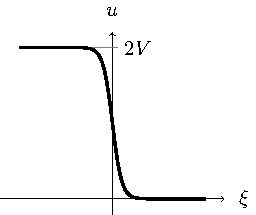
\includegraphics[scale=1.5]{img/shock_waves/shock_knot}}
\end{minipage}
	% \caption{Зависимость $\Re p$ от $k^2$ при $D_{1,2}\ne0$ и структура Тьюринга (справа)}
\end{figure}
% Здесь не будет осцилляций. Во всех случаях есть передний фронт.
